\chapter{Některé příkazy balíčku \texttt{thesis}}\label{priloha:A}

\section{Příkazy pro sazbu veličin a jednotek}

\begin{table}[!h]
  \caption{Přehled příkazů pro matematické prostředí }
  \begin{center}
  	\small
	  \begin{tabular}{|c|c|c|c|}
	    \hline
	    Příkaz    						& Příklad 					& Zdroj příkladu  							& Význam  \\
	    \hline\hline
	    \verb|\textind{...}|	& $\beta_\textind{max}$ 	& \verb|$\beta_\textind{max}$|	& textový index \\
	    \hline
	    \verb|\konst{...}| 		& $\konst{U}_\textind{in}$ 				& \verb|$\konst{U}_\textind{in}$|		& konstantní veličina \\
	    \hline
	    \verb|\prom{...}| 		& $\prom{u}_\textind{in}$ & \verb|$\prom{u}_\textind{in}$| & proměnná veličina \\
	    \hline
	    \verb|\komplex{...}| 	& $\komplex{u}_\textind{in}$ & \verb|$\komplex{u}_\textind{in}$| & komplexní veličina \\
	    \hline
	    \verb|\vekt{...}| 		& $\vekt{y}$ 						& \verb|$\vekt{y}$| & vektor \\
	    \hline
	    \verb|\matice{...}| 	& $\matice{Z}$ 						& \verb|$\matice{Z}$| & matice \\
	    \hline
	    \verb|\jedn{...}| 		& $\jedn{kV}$ 						& \verb|$\jedn{kV}$|\quad či\ \, \verb|\jedn{kV}| & jednotka \\
	    \hline
	  \end{tabular}
  \end{center}
\end{table}



%\newpage
\section{Příkazy pro sazbu symbolů}

\begin{itemize}
  \item
    \verb|\E|, \verb|\eul| -- sazba Eulerova čísla: $\eul$,
  \item
    \verb|\J|, \verb|\jmag|, \verb|\I|, \verb|\imag| -- sazba imaginární jednotky: $\jmag$, $\imag$,
  \item
    \verb|\dif| -- sazba diferenciálu: $\dif$,
  \item
    \verb|\sinc| -- sazba funkce: $\sinc$.
  \item
    \verb|\mikro| -- sazba symbolu mikro stojatým písmem\footnote{znak pochází z~balíčku \texttt{textcomp}}: $\mikro$.

\end{itemize}
%
Všechny symboly jsou určeny pro matematický mód, vyjma \verb|\mikro|, jenž je použitelný rovněž v~textovém módu.






\chapter{Osazené DPS}\label{priloha:B}


\section{Testovací DPS C}
\begin{figure}[H]
  \centering
    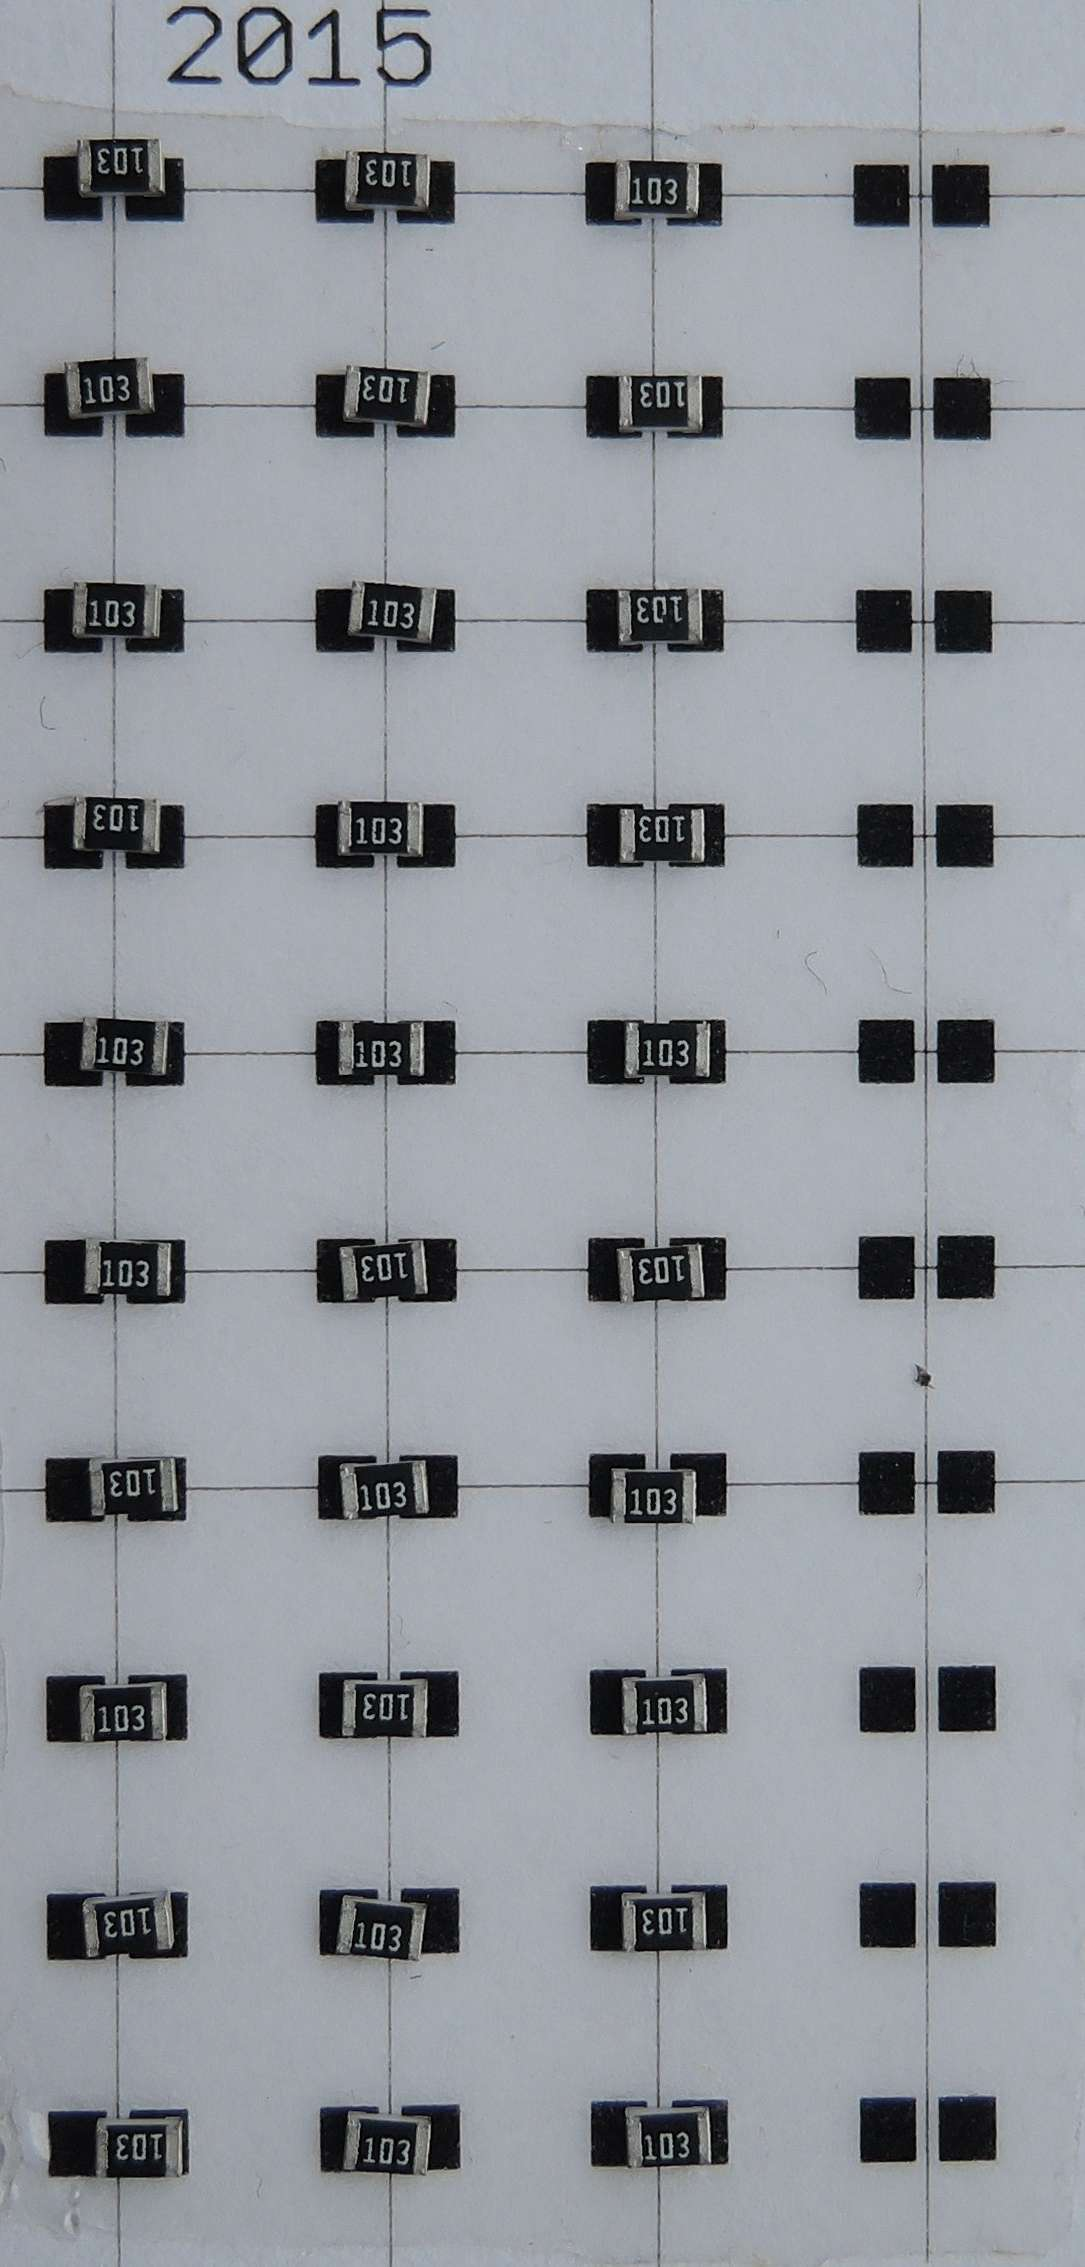
\includegraphics[height=0.35\paperheight ]{obrazky/C2.jpg}%
    \caption{Testovací DPS C.}
    \label{img:DeskaC}
\end{figure}


\begin{table}[H]
  \caption{Naměřené chyby osazení pro testovací DPS C.}
  \begin{center}
  	\small
	  \begin{tabular}{|c|c|c|c|c|c|c|c|c|c|c|}
	    \hline
			& \textbf{R41}	& \textbf{R42}	& \textbf{R43}	& \textbf{R44}	& \textbf{R45}	& \textbf{R46}	& \textbf{R47}	& \textbf{R48}	& \textbf{R49}	& \textbf{R50}  \\
	    \hline
	    \textbf{x}	& 0,455&	0,364&	0,242&	0,364&	0,121&	0,091&	0,091&	0,030&	0,182&	0,06  \\
	    \hline
	    \textbf{y}	&0,212&	0,091&	0,182&	0,061&	0,364&	0,455&	0,545&	0,273&	0,212&	0,515 \\
	    \hline
			& \textbf{R51}	& \textbf{R52}	& \textbf{R53}	& \textbf{R54}	& \textbf{R55}	& \textbf{R56}	& \textbf{R57}	& \textbf{R58}	& \textbf{R59}	& \textbf{R60}  \\
	    \hline
	    \textbf{x}	&0,182&	0,212&	0,212&	0,212&	0,182&	0,000&	-0,030&	0,030&	-0,152&	0,061  \\
	    \hline
	    \textbf{y}	&0,091&	0,030&	0,303&	-0,061&	-0,030&	0,030&	-0,061&	-0,061&	-0,182&	0,030 \\
	    \hline
	    		& \textbf{R61}	& \textbf{R62}	& \textbf{R63}	& \textbf{R64}	& \textbf{R65}	& \textbf{R66}	& \textbf{R67}	& \textbf{R68}	& \textbf{R69}	& \textbf{R70}  \\
	    \hline
	    \textbf{x}	& -0,030&	0,000&	0,061&	0,000&	0,000&	-0,061&	-0,333&	-0,030&	0,030&	-0,061 \\
	    \hline
	    \textbf{y}	& 0,000&	0,030&	-0,030&	0,000&	-0,152&	0,000&	-0,091&	0,061&	0,182&	0,152 \\
	    \hline
	  \end{tabular}
  \end{center}
\end{table}




\section{Testovací DPS D}
\begin{figure}[H]
  \centering
    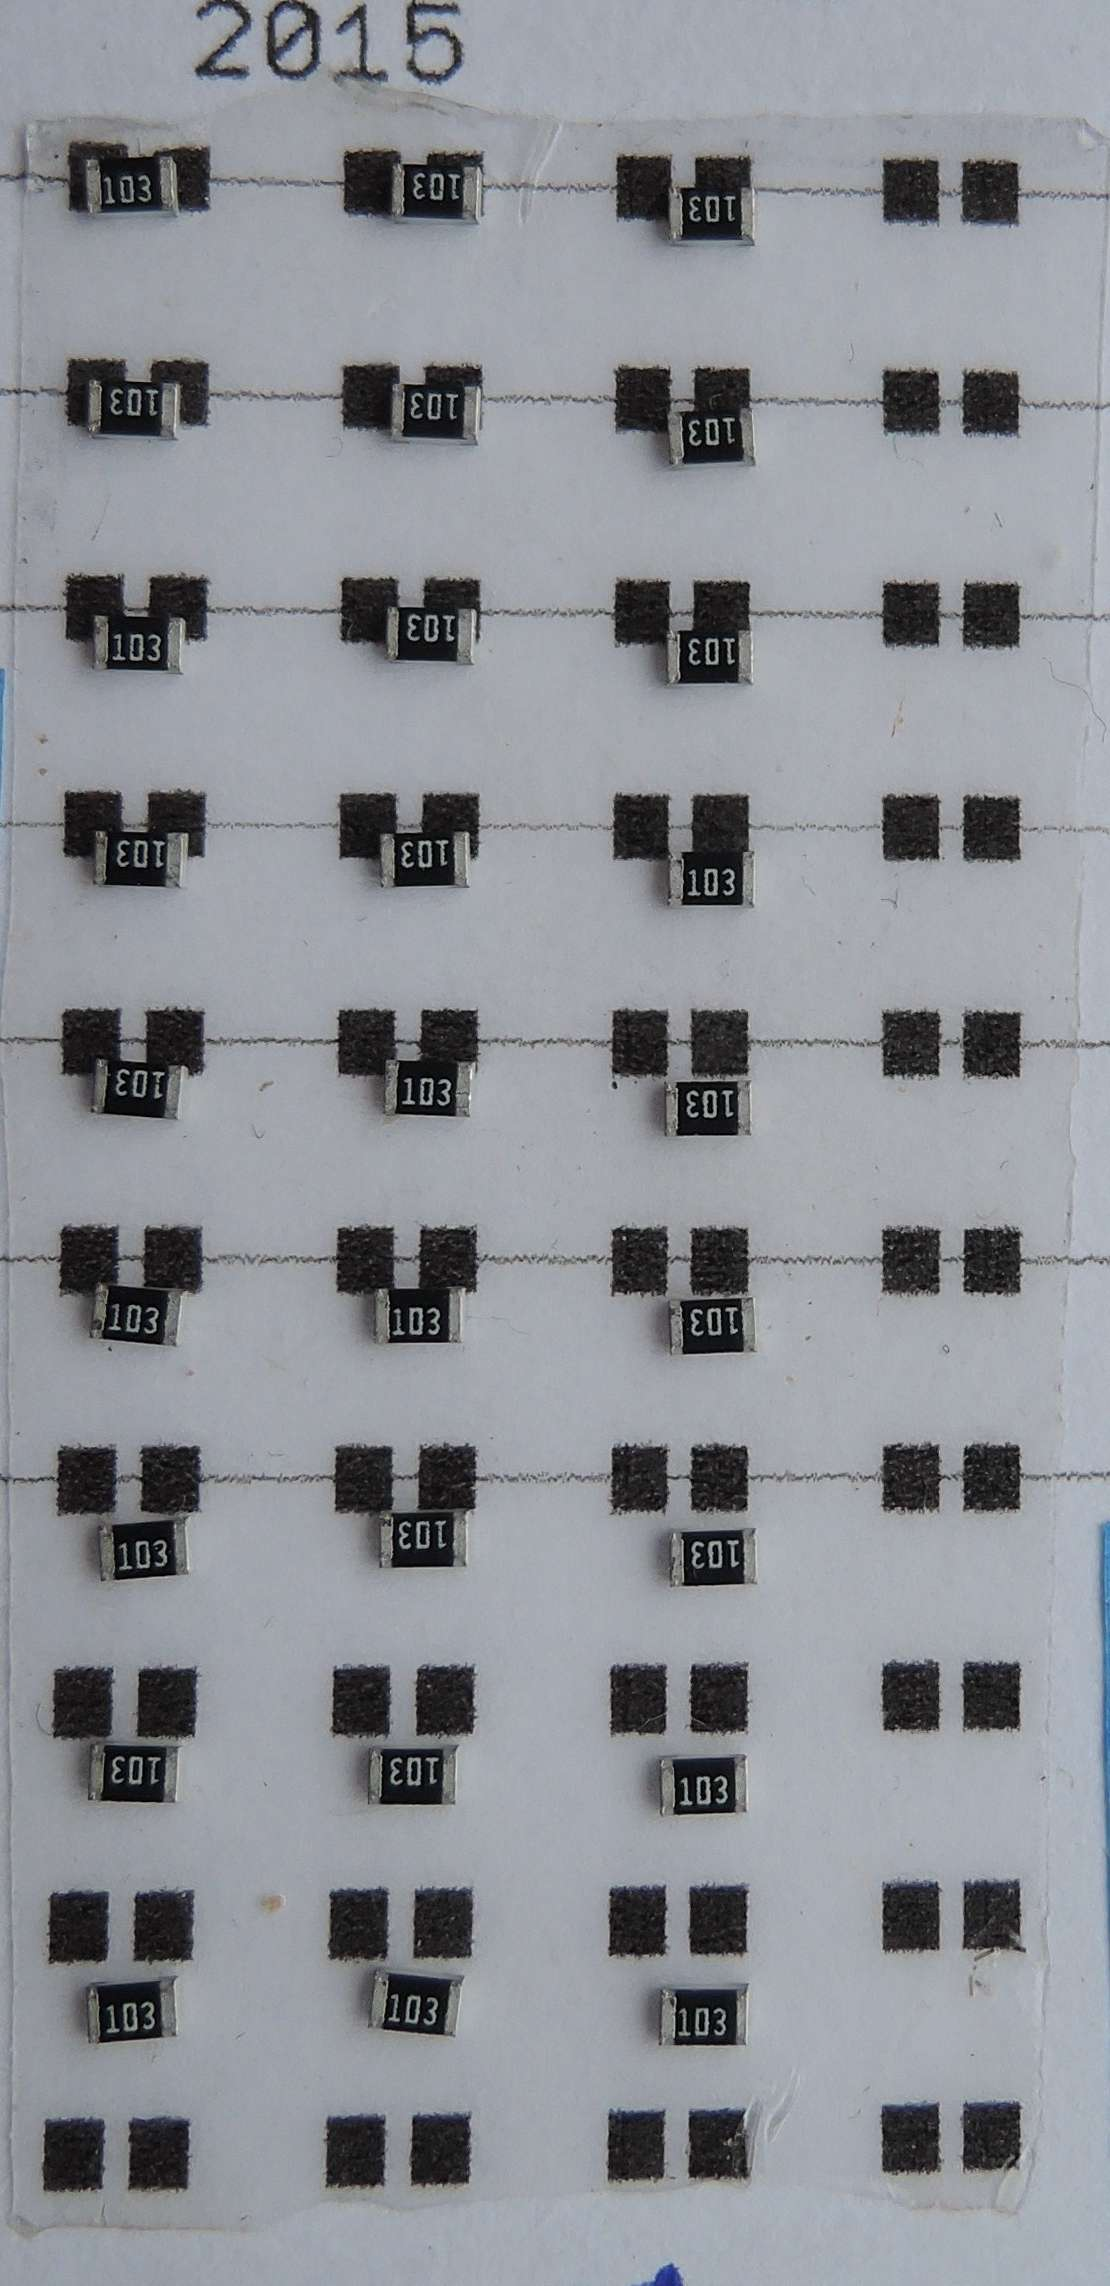
\includegraphics[height=0.35\paperheight ]{obrazky/D2.jpg}%
    \caption{Testovací DPS D.}
    \label{img:DeskaD}
\end{figure}


\begin{table}[H]
  \caption{Naměřené chyby osazení pro testovací DPS D.}
  \begin{center}
  	\small
	  \begin{tabular}{|c|c|c|c|c|c|c|c|c|c|c|}
	    \hline
			& \textbf{R41}	& \textbf{R42}	& \textbf{R43}	& \textbf{R44}	& \textbf{R45}	& \textbf{R46}	& \textbf{R47}	& \textbf{R48}	& \textbf{R49}	& \textbf{R50}  \\
	    \hline
	    \textbf{x}	& -0,515&	-0,485&	-1,121&	-0,818&	-1,121&	-1,424&	-1,758&	-1,576&	-1,970&	na \\
	    \hline
	    \textbf{y}	&-0,182&	-0,182&	0,212&	0,030&	0,061&	0,242&	0,576&	0,182&	0,455&	na \\
	    \hline
			& \textbf{R51}	& \textbf{R52}	& \textbf{R53}	& \textbf{R54}	& \textbf{R55}	& \textbf{R56}	& \textbf{R57}	& \textbf{R58}	& \textbf{R59}	& \textbf{R60}  \\
	    \hline
	    \textbf{x}	& -0,424&	-0,455&	-0,545&	-0,848&	-1,273&	-1,485&	-1,364&	-1,697&	-1,939&	na  \\
	    \hline
	    \textbf{y}	& 0,545&	0,545&	0,485&	0,333&	0,515&	0,242&	0,364&	0,182&	0,394&	na \\
	    \hline
	    		& \textbf{R61}	& \textbf{R62}	& \textbf{R63}	& \textbf{R64}	& \textbf{R65}	& \textbf{R66}	& \textbf{R67}	& \textbf{R68}	& \textbf{R69}	& \textbf{R70}  \\
	    \hline
	    \textbf{x}	& -0,727&	-1,030&	-1,152&	-1,394&	-1,667&	-1,606&	-1,970&	-2,091&	-2,182&	na \\
	    \hline
	    \textbf{y}	& 0,636&	0,667&	0,667&	0,788&	0,636&	0,758&	0,758&	0,636&	0,667&	na \\
	    \hline

	  \end{tabular}

  \end{center}

\end{table}







\section{Testovací DPS E}
\begin{figure}[H]
  \centering
    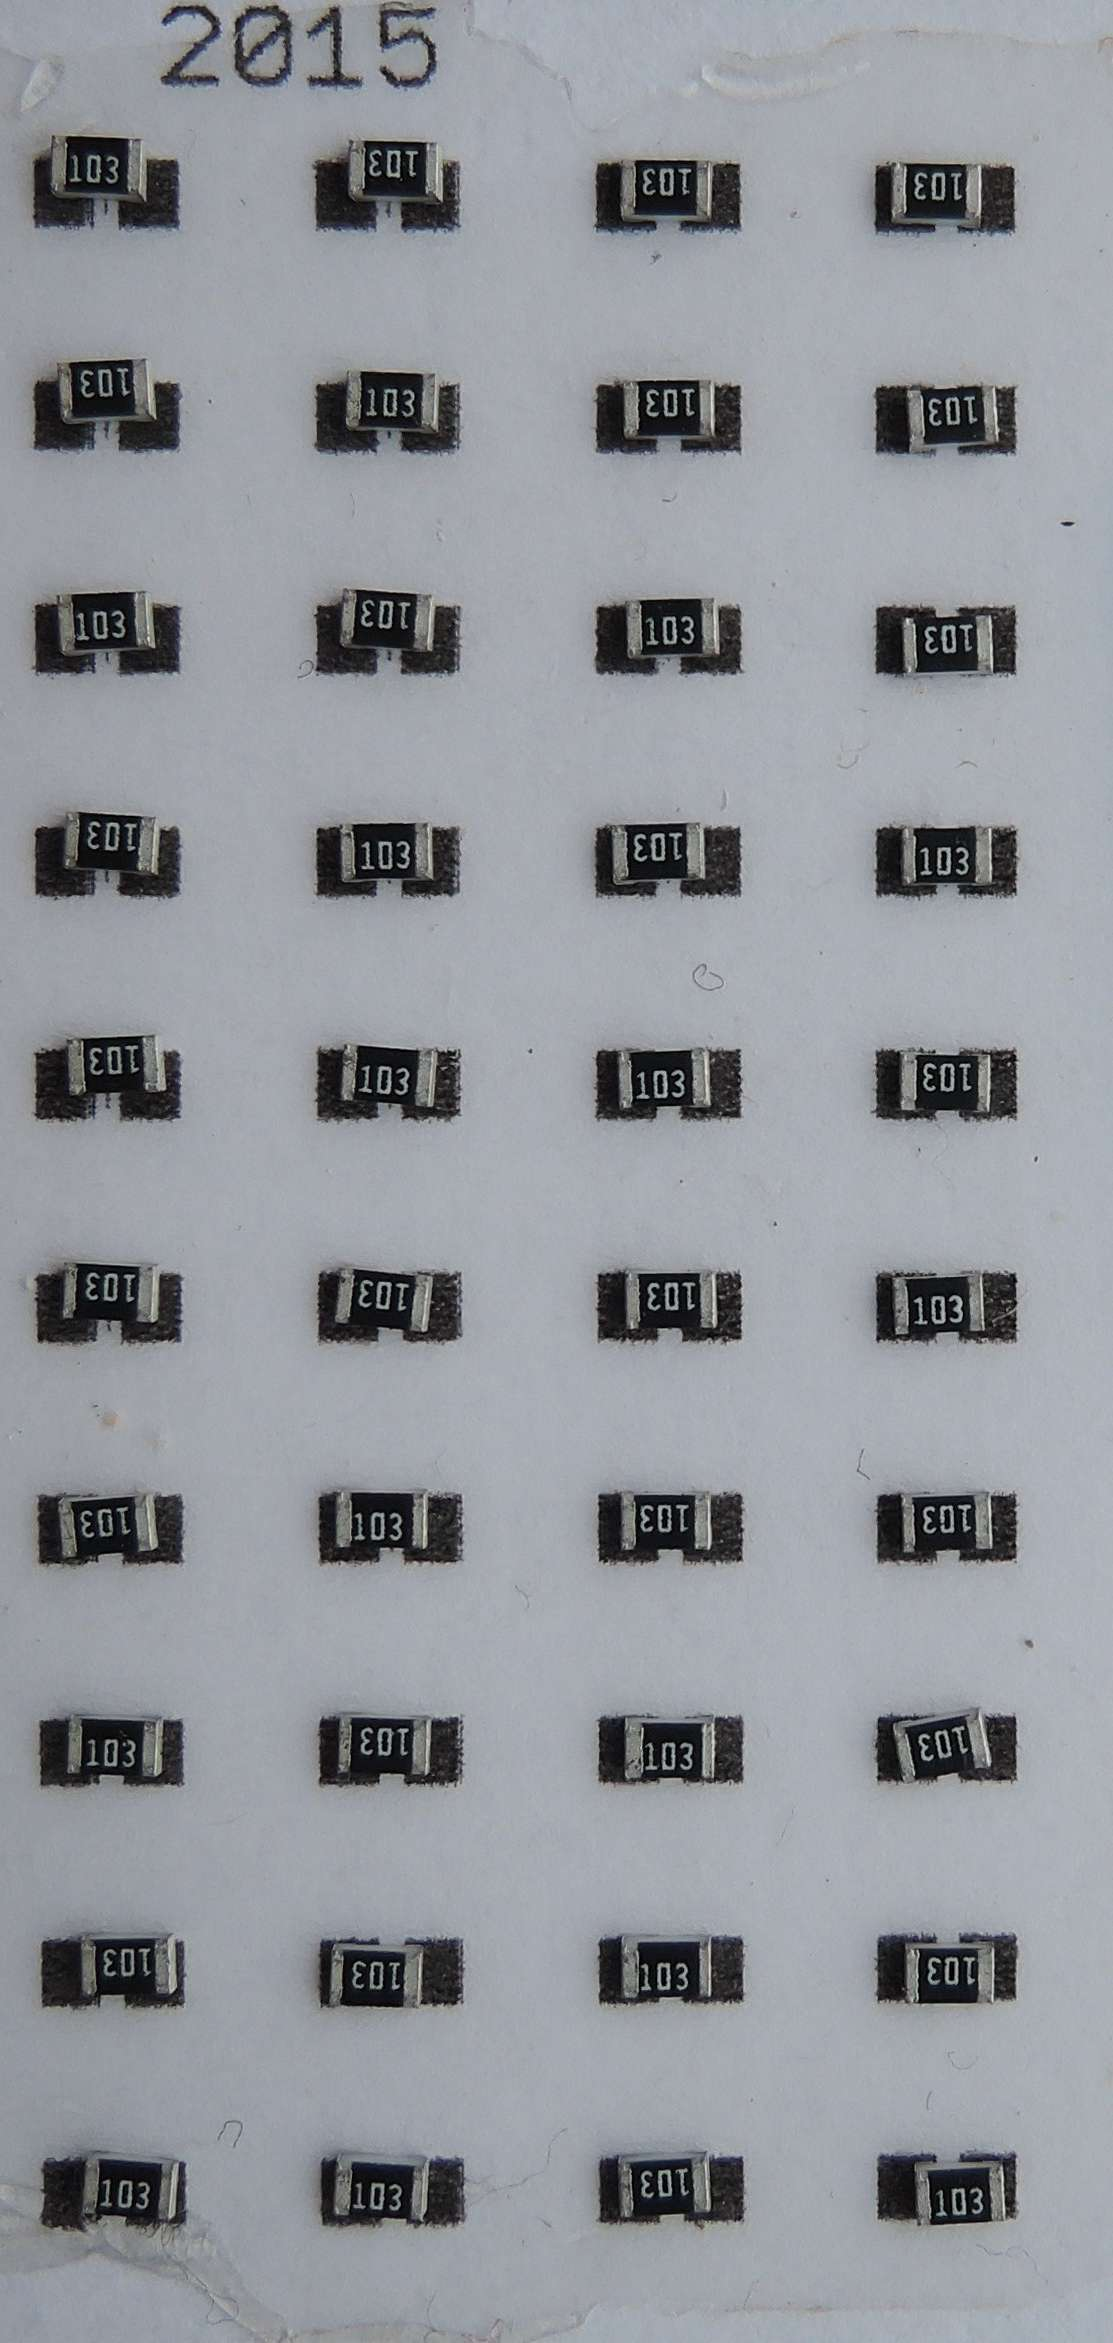
\includegraphics[height=0.35\paperheight ]{obrazky/E2.jpg}%
    \caption{Testovací DPS E.}
    \label{img:DeskaE}
\end{figure}



\begin{table}[H]
  \caption{Naměřené chyby osazení pro testovací DPS E.}
  \begin{center}
  	\small
	  \begin{tabular}{|c|c|c|c|c|c|c|c|c|c|c|}
	    \hline
			& \textbf{R41}	& \textbf{R42}	& \textbf{R43}	& \textbf{R44}	& \textbf{R45}	& \textbf{R46}	& \textbf{R47}	& \textbf{R48}	& \textbf{R49}	& \textbf{R50}  \\
	    \hline
	    \textbf{x}	& 0,515	& 0,515	& 0,424	& 0,394	& 0,485	& 0,515	& 0,303	& 0,273	& 0,333	& 0,333 \\
	    \hline
	    \textbf{y}	&-0,030	& 0,242	& 0,091	& 0,212	& 0,364	& 0,303	& -0,030 & 0,273 & 0,515& 0,576 \\
	    \hline
			& \textbf{R51}	& \textbf{R52}	& \textbf{R53}	& \textbf{R54}	& \textbf{R55}	& \textbf{R56}	& \textbf{R57}	& \textbf{R58}	& \textbf{R59}	& \textbf{R60}  \\
	    \hline
	    \textbf{x}	& 0,545	& 0,333	& 0,515	& 0,182	& 0,242	& 0,333	& 0,333	& 0,333	& 0,091	& 0,242  \\
	    \hline
	    \textbf{y}	& 0,333	& 0,273	& 0,152	& 0,061	& -0,030& -0,182& -0,242& -0,152& -0,364& -0,242 \\
	    \hline
	    		& \textbf{R61}	& \textbf{R62}	& \textbf{R63}	& \textbf{R64}	& \textbf{R65}	& \textbf{R66}	& \textbf{R67}	& \textbf{R68}	& \textbf{R69}	& \textbf{R70}  \\
	    \hline
	    \textbf{x}	& 0,000	& 0,152	& 0,212	& 0,333	& 0,121	& 0,273	& 0,242	& 0,030	& 0,061	& -0,333 \\
	    \hline
	    \textbf{y}	& 0,000	& -0,030& 0,121	& -0,273& 0,000	& -0,061& 0,030	& 0,000	& 0,000	& 0,212 \\
	    \hline

	  \end{tabular}

  \end{center}

\end{table}


\chapter{Obsah přiloženého CD}\label{priloha:C}

Nezapomeňte uvést, co čtenář najde na přiloženém médiu.
Je vhodné okomentovat obsah každého adresáře, specifikovat, který soubor obsahuje důležitá nastavení, který soubor je určen ke spuštění atd.
Také je dobře napsat, v~jaké verzi software byl kód testován (např.\ Matlab 2010b).
